\documentclass{amia}
\usepackage{graphicx}
\usepackage[labelfont=bf]{caption}
\usepackage[superscript,nomove]{cite}
\usepackage{color}
\usepackage{multirow}
\renewcommand*{\thefootnote}{\fnsymbol{footnote}}

\begin{document}

\title{Machine Learning Models for the Segmentation of eCoaching Text}

\author{Mehedi Hasan, BS$^{1}$\footnote[1]{Authors provided equal contribution. \label{footnote1}}, Alexander Kotov, PhD$^{1}$\textsuperscript{\ref{footnote1}}, April Idalski Carcone, PhD$^{2}$, Ming Dong, PhD$^{1}$, Sylvie Naar, PhD$^{2}$}

\institutes{
$^1$Department of Computer Science, Wayne State University, Detroit, Michigan \\  
$^2$Department of Family Medicine and Public Health Sciences, School of Medicine, Wayne State University, Detroit, Michigan\\
}

\maketitle

\noindent{\bf Abstract}
\textit{Machine learning-based models has the potential to to efficiently and accurately identify patient-provider communication behaviors during eCoaching intervention sessions targeting fruit and vegetable intake among young adults age 21-30. }

1) Motivation: Why do we care about the problem and the results? \\
2) Problem statement: What problem is the paper trying to solve and what is the scope of the work? \\
3) Approach: What was done to solve the problem? \\
4) Results: What is the answer to the problem? \\
5) Conclusions: What implications does the answer imply?

\section*{Introduction}
Unhealthy eating habits, particularly low fruit and vegetable intake, is a growing, serious public health concern, particularly among young adults age 21-30, referred to as Generation Y (GenY)\cite{blanck2008trends,centers2007fruit}. This generation has adopted a lifestyle that involves eating accessible, ``no mess'', quick, ``grab and go'' foods\cite{nebeling2007still,brug1999application}. They mainly eat ``out'' and infrequently shop and prepare food, limiting access to fruit and vegetables (FV)\cite{nelson2009improving,larson2006food}. Unfortunately, less than one-third of US adults\cite{blanck2008trends,ogden2006prevalence} and only 20\% of GenY\cite{blanck2008trends,american2006american,thompson2005dietary} eat the recommended 5 servings of fruit and vegetables daily. Those in inner city urban and rural settings have among the poorest eating habits\cite{blanck2008trends,centers2007fruit,ogden2006prevalence,american2006american,thompson2005dietary}. GenY's poor dietary practices placing them at high risk for obesity and many chronic diseases, such as type 2 diabetes, as well as declines in predicted health status and life expectancy. Thus, there is a need to develop effective interventions to improve GenY's eating habits.

GenY is a tech-savvy generation requiring an intervention matched to their mobile lifestyle. Growing numbers use the internet to access health information with the largest increases in internet access among low-income Americans, making the internet well-suited for health promotion intervention\cite{strecher2007internet}. MENU GenY\cite{alexander2017motivations} (Making Effective Nutrition Choices for Generation Y) is a technology-based public health intervention to encourage increased fruit and vegetable intake among GenY. A critical component of MENU GenY is personalized eCoaching. eCoaches use email to deliver motivation-enhancing coaching to encourage healthy eating, grounded in the principles of Motivational Interviewing (MI), an evidence-based communication technique to increase intrinsic motivation and self-efficacy for behavior change\cite{miller2012motivational,miller2009ten,miller2009toward}. Patient ``change talk'', statements of intrinsic motivation about their desire, ability, reasons, need for and commitment to behavior change, is an established mediator of health behavior change\cite{apodaca2009mechanisms}. Identifying specific communication strategies linked to behavior change and integrating these strategies into communication-based interventions (e.g., brief, motivation-enhancing interventions delivered in a variety of settings or public health initiatives) can increase these interventions' potency.

A major drawback of this research is the qualitative methods traditionally used to analyze the communication process which are resource-intensive, requiring an iterative process of human (subjective) interpretation of text. Rapidly developing computational technologies, specifically machine learning combined with classification models, offer a unique opportunity to accelerate this process. Our research group has recently applied machine learning-based models to similar communication data\cite{hasan2016study,kotov2015interpretable}. A simple communication code scheme was automated to characterize patient communication and achieved accuracy comparable to human coders\cite{hasan2016study}. The ultimate goal of the research study is to leverage innovative machine learning models to fully automate the communication coding process in eCoach-patient communication to increases in fruit and vegetable intake. 

However, a significant barrier of fully automate eCoaching is the unsegmented text data. Developing an automatic classification of clinical interactions required segmented text. Nevertheless, eCoaching data comprised of email responses which need to be segmented into group of MI behavior referes to ``block of text''. Automatic segementation of eCoaching intervention sessions is a challenging task due to the 2 important reasons. First, the email is an unstructured text that contains informal email exchange in non-traditional formats. Second, a text segment not necessarily belongs to the entire sentence or collection of sentences. One sentence can be segmented into several MI behaviors, and vice versa. Figure 1 illustrates that the marked sentence taken from an eCoaching email exchanage, segmented into 2 different MI behaviors, CHT and HUP. 

In this paper, we address this problem by developing several state-of-the-art machine learning based models for the segmentation of eCoaching text to promote the automatic identification of best communication strategies without human interference. More specifically, we develop Support Vector Machine (SVM), Naive Bayes (NB), K-Nearest Neighbor (KNN), Long Short Term Memory (LSTM), and Gated Recurrent Unit (GRU) by utlizing contextual, topic and punctuation mark features, to find the best model for the segmentation of eCoaching text. 

Previous studies mainly focus on segemntation of text into sections and headers\cite{apostolova2009automatic,denny2009evaluation,tepper2012statistical,cho2002text} or sentence boundary detection\cite{griffis2016quantitative,kreuzthaler2015detection,treviso2016sentence} in the medical domain. Apostolova et al.\cite{apostolova2009automatic} applied SVM by utilizing word-vector cosine similarity metric combined with several heuristics to classify clinical report into semantic sections such as demographics, history, exam procedure, finding, impression, etc. After identification of each line in the document, Tepper et al. \cite{tepper2012statistical} trained an Maximum Entrophy models for the section classification. In 2009, Denny et al.\cite{denny2009evaluation} proposed a SecTag algorithm, which combined natural language processing technique, terminology-based rule, and naive bayesian score for identifying sections and headers that achieved 99\% recall with 95.6\% precision. On the other hand, SVM exploiting with linear kernel and recurrent convolutional neural networks with posodic, part of speech features and word embeddings, were trained by Kreuzthaler et al.\cite{kreuzthaler2015detection} and Griffis et al.\cite{griffis2016quantitative}, respectively, for the detection of sentence boundary. However, segmentation of clinical text, in partiicular, segmentation of MI or eCoaching text into group of MI behavior is ignored while relying on manual hand-coded approach. Therefore, this study introduce an innovative approach and the authors are not aware of any other work this approach has been considered for the segmentation of MI or eCoaching text into ``block of text''. 

\section*{Methods}
\subsection*{\textit{Data collection}}
The experimental dataset for this work was constructed from the transcripts of 129 motivational interviews, which include a total of 50,239 segmented and annotated utterances. Each transcript consists
of an MI interview session involving counselor, adolescent, and caregiver. The utterances were annotated based on MYSCOPE codebook \cite{carcone2013provider}, in which the codes are grouped into
patient (adolescent and caregiver) codes and counselor codes. Utterances were divided into successful and unsuccessful communication sequences. Successful communication sequences result in
positive change talk and commitment language statements by an adolescent or caregiver, while unsuccessful sequences are the ones that result in negative change talk or commitment language and the
sequences, in which no change talk or commitment language statements occur. Out of 5143 observed sequences, 4225 were positive and 918 were negative. Successful sequences had an average length of
9.79 utterances, while unsuccessful sequences had on average 9.65 utterances. For each of the probabilistic models (MC and HMM), two models were trained, one model was trained using successful
sequences and another one was trained using unsuccessful sequences. 

Part 1

1) What algorithms or data structures did you select? Who created them? What is their asymptotic behavior? What other specific characteristics are worth noting for this study?\\
2) What programming language and platform did you use? What impact did these choices have on your project?\\


Part 2

1) How specifically did you implement the algorithms?\\
2) How did you handle instrumentation code? Why?\\
3) Did you perform any optimizations? Why or why not?\\
4) How did you choose to test and benchmark your code?\\
5) What inputs (data) did you select to test your implementations? Why?\\

\subsection*{\textit{Segmentation method}}
Generally, a sequence can be viewed as a temporally ordered set of events. In this study, an event is a behavior code that also has a symbolic representation.

\textbf{Naive Bayes}: comming soon...

\textbf{Support Vector Machine}: comming soon...

\textbf{K-Nearest Neighbour}: comming soon...

\textbf{Recurrent Neural Networks}: comming soon...
  
\subsection*{\textit{Evaluation metrics}}
Performance of the proposed method was evaluated in terms of precision, recall, and F-measure using 10 folds cross-validation and weighted macro-averaging of these metrics over the folds. However, LSTM and GRU are trained on 80\% of the data and validated on 10\%. The remaining 10\% of the data is used as a test set for reporting the performance of the model. 

\section*{Results}
Experimental evaluation of the proposed method is conducted on both under and over-sampled sequences. Predictive performance summary of the proposed methods on under and over-sampled sequences is presented in Table.\\

1) In general, the pure, unbiased results should be presented first without interpretation (van Wagenen 1990). \\
2) These results should present the raw data
or the results after applying the techniques outlined in the methods section. The results are simply results; they do not draw conclusions.

\begin{table}[ht]
\centering
\caption{Performance of NB, SVM, KNN, and RNN for identifying segmentation point in eCoaching text. The highest value for each performance metric is highlighted in bold.}
\label{tab:result_under_over_sampled}
  \begin{tabular}{|l|l|l|l|l|l|l|}
  \hline
   \multirow{2}{*}{\textbf{Method}} & \multicolumn{3}{|c|}{\textbf{contextual features only}} & \multicolumn{3}{|c|}{\textbf{contextual + topics + punctuation marks}} \\\cline{2-7}
   & \textbf{Precision}  & \textbf{Recall} & \textbf{F1-Score} & \textbf{Precision}  & \textbf{Recall} & \textbf{F1-Score}\\ \hline    
    
 Naive Bayes Multinomial & 0.594 & 0.662 & 0.626 & 0.590 & 0.666 & 0.626 \\ \hline
 Support Vector Machine & 0.742 & \textbf{0.679} & 0.709 & 0.774 & 0.696 & 0.733\\ \hline
 K-Nearest Neighbour & \textbf{0.808} & 0.663 & \textbf{0.728} & \textbf{0.820} & \textbf{0.742} & \textbf{0.779}\\ \hline
 Long Short Term Memory & 0.8424 & 0.8385 & 0.8381 & 0.8424 & 0.8385 & 0.8381\\ \hline
 Gated Recurrent Unit & 0.8705 & 0.8676 & 0.8673 & 0.8412 & 0.8377 & 0.8373\\ \hline 
  \end{tabular}
\end{table} 

Predictive performance summary of the proposed methods on under and over-sampled sequences is presented in Table.\\

\begin{table}[ht]
\centering
\caption{Performance of NB, SVM, KNN, and RNN for identifying continuous eCoaching text. The highest value for each performance metric is highlighted in bold.}
\label{tab:result_under_over_sampled}
  \begin{tabular}{|l|l|l|l|l|l|l|}
  \hline
   \multirow{2}{*}{\textbf{Method}} & \multicolumn{3}{|c|}{\textbf{contextual features only}} & \multicolumn{3}{|c|}{\textbf{contextual + topics + punctuation marks}} \\\cline{2-7}
   & \textbf{Precision}  & \textbf{Recall} & \textbf{F1-Score} & \textbf{Precision}  & \textbf{Recall} & \textbf{F1-Score}\\ \hline    
    
 Naive Bayes Multinomial & 0.988 & 0.985 & 0.987 & 0.989 & 0.984 & 0.986 \\ \hline
 Support Vector Machine & \textbf{0.989} & 0.992 & 0.991 & 0.990 & 0.993 & 0.991\\ \hline
 K-Nearest Neighbour & \textbf{0.989} & \textbf{0.995} & \textbf{0.992} & \textbf{0.991} & \textbf{0.994} & \textbf{0.993}\\ \hline
 Long Short Term Memory & 0.8424 & 0.8385 & 0.8381 & 0.8424 & 0.8385 & 0.8381\\ \hline
 Gated Recurrent Unit & 0.8705 & 0.8676 & 0.8673 & 0.8412 & 0.8377 & 0.8373\\ \hline 
  \end{tabular}
\end{table} 

We took the inspiration for the representation of behavior codes from the idea of word embeddings. Word embedding is a representation of words in
low-dimensional space by vectors, which contain the features of the words. In our study, we employed embedding in place of one-hot vectors for representation of behavior codes as input to LSTM and
GRU, since one-hot vectors are high-dimensional and sparse. 

\begin{figure}[!htb]
    \centering
    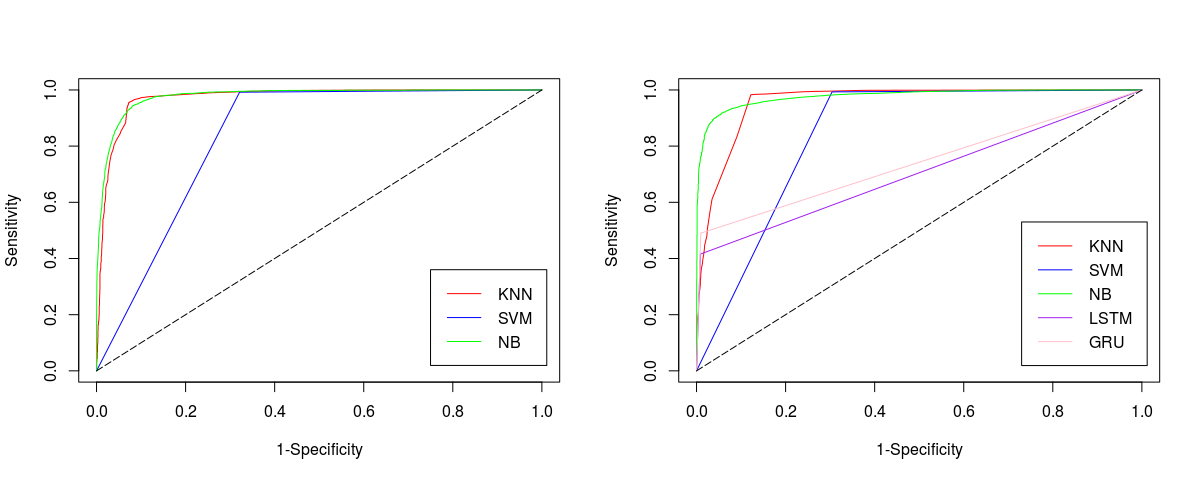
\includegraphics[width=1.0\textwidth]{figures/roc-curves.png}
    \caption{\textbf{ROC curves compared the performance of different models}.}
    \label{fig:roc-curves}
\end{figure}

\section*{Discussion}
By analyzing the experimental results of different communication sequence outcome prediction methods proposed in this paper, we arrived at the following conclusions. First, the overall predictive
performance of RNN models is substantially better than probabilistic models. In particular, the RNN-based method achieves near-human accuracy for predicting the 


1) What, specifically, did you learn from comparing these algorithms or data structures? \\
2) What do your results say about the problem or question you were investigating?\\
3) Was your hypothesis confirmed or disproved?\\
4) Are the results what you expected?\\
5) If you obtained anomalies or other unexpected results, can you explain them? If not, how could you set about in the future to identify what caused them? \\
6) How do your results compare to past findings? Are they consistent? Different?Why? \\
7) How would you respond to objections or questions that other researchers might have about your methods, results, or interpretations? \\
8) What is new and significant?\\
 
\section*{Conclusion}
In this paper, we compared the performance of machine learning models for the task of segmentation of e-coaching text. We found out that k-nearest neighbour provides the best performance for the segmentaion of text in terms of all performance metrics. Manual segmentation of e-coaching data is very resource-intensive and time consuming task, which can significantly decrease the time and effort required to develop effective behavioral interventions. Our
proposed methods can help to identify individual text segments, which can be annotated directly with a classification model and increase the effectiveness of behavioral interventions. This approach will help for developing fully automated eCoaching and also accelerate the pace of identifying effective communication strategies linked to healthy eating.  

1) The hypothesis and the evidence for and against it are briefly restated \\
2) The original motivation is recapitulated \\
3) The state of the field in the light of this new contribution is reassessed \\
4) describes future research and new directions suggested by the contribution\\
5) in particular, research that would improve the evidence for or against the hypothesis

\section*{Acknowledgments}
This study was supported by a grant from the National Institutes of Health, NIDDK R21DK108071, Carcone and Kotov, MPIs. We would like to thank the student assistants in the Department of Family Medicine and Public Health Sciences at Wayne State University School of Medicine for their help in developing the training dataset by manually annotating the dataset using the MYSCOPE codebook. 

\bibliographystyle{vancouver}
\bibliography{references}

\end{document}
